% Compilare con PDFLaTeX
\documentclass[10pt,final]{siamltex}
\usepackage{graphicx}
\usepackage{latexsym}
\usepackage{amsmath,amssymb}
%\usepackage{gensymb}
\textwidth = 16cm
\usepackage{pstricks}
%\usepackage{subcaption}
\usepackage{algorithm}
\usepackage{algpseudocode}
\usepackage[breakable]{tcolorbox}
\usepackage{doi}
\usepackage{caption}%http://ctan.org/pkg/caption
\captionsetup[table]{format=plain,labelformat=simple,labelsep=period}

\usepackage[framed,numbered,autolinebreaks,useliterate]{mcode}

%
\begin{document}
\title{Glomerular filtration rate estimation by a novel binning-less bivariate isotonic statistical regression method}
\author{Sebastian~Giles, Simone~Fiori%
\thanks{S. Giles is with the School of Information and Automation Engineering,
Universit\`{a} Politecnica delle Marche,
Via Brecce Bianche, I-60131 Ancona (Italy).
\newline\indent
S. Fiori is with Dipartimento di Ingegneria dell'Informazione,
Universit\`{a} Politecnica delle Marche,
Via Brecce Bianche, I-60131 Ancona (Italy).
\newline\indent
This draft is dated \today.}}
\maketitle
\def\bbbr{\mathbb{R}}
\def\bbbx{\mathbb{X}}
\def\bbby{\mathbb{Y}}
\def\mdef{{\stackrel{{\mathrm{def}}}{=}}}
% Footnotes in non-numerical fashion
\renewcommand*{\thefootnote}{\fnsymbol{footnote}}
\def\to{\mathbf{\ to\ }}
\setcounter{footnote}{1}
%
%
\begin{abstract}
  Bivariate statistical regression is a method for finding a relationship between unpaired sets of data based on statistic distribution matching. In the present report, an efficient numerical algorithm is proposed to perform bivariate regression. The method is then applied to correlate glomerular filtration rate to serum creatinine concentration. Glomerular filtration rate is an important indicator of kidney function. As direct measurement is highly impractical, there is considerable interest in developing numerical algorithms to estimate glomerular filtration rate from parameters which are easier to obtain, such as demographic data and `bedside' assays results.
\end{abstract}
%
\section{Introduction}\label{intro}
Several real-world complex phenomena in vistually any branch of science lack accurate mathematical descriptions \cite{seismic,strontium}. In these cases, it is not possible to predict the value of a variable by plugging known quantities into an analytically derived expression, therefore, empirical methods must be employed to develop a model of the observed process. The most common set of tools used to infer a functional relationship between variables is regression analysis \cite{control, ts}.

%Here only bivariate regression techniques will be considered. The amount of available data is assumed to be enough to explain the relevant statistical features of the phenomenon underlying the data.

The problem that triggered the present research is the estimation of glomerular filtration rate (GFR), which is used as an indicator of kidney function and is relevant for assessing progression of renal disease. It is also frequently required for evaluating optimal dosage for medications \cite{gfrmed,gfralb}. However, determination of true GFR is time-consuming, costly, and difficult to perform \cite{mgfr2,mgfr}. Thus, there is considerable interest in developing models to estimate GFR using simpler parameters such as age, weight, height, gender and values which can be more conveniently measured as part of a typical blood test.

Traditional forms of regression are based on some parametrised function whose graph is made to lay reasonably close to the points making up the experimental dataset. Values for the parameters are typically found using the least squares method \cite{book}.

Isotonic regression allows greater freedom for the regression curve to fit data by constructing a piecewise linear function, described by a lookup table (LUT). Overfitting is avoided by requiring the function to be monotonic, which is reasonable whenever the underlying physical phenomenon is inherently monotonic (such as the relationship between percentage body fat and waist circumference \cite{fat}). Various algorithms can be used to find the LUT values that satisfy a least squares condition \cite{bestchak, pava}.

Statistical bivariate regression (SBR) constitutes an improvement over isotonic regression. Its advantages derive from the fact that it relies on finding the relationship between the statistical distributions of the variables. SBR is not based on a least squares method so it does not require data to be associated in ordered pairs. This makes it ideal for correlating two quantities that cannot be both measured on the same individual. The algorithm presented in \cite{fiori} independently estimates the probability density functions (PDF) of the two variables by dividing the dataset ranges into bins and populating look-up tables (LUTs) for the relative frequencies. The PDFs are then integrated to obtain the cumulative distribution functions (CDF) which are, or can be licitly adjusted to be, bijective and allow for the regression model to be obtained as the map between values with equal probabilities.

This report describes an alternative algorithm developed to make bivariate statistical regression more versatile and faster over large datasets by entirely avoiding the binning (previously required to estimated PDFs) and numerical integration operations (previously required to estimated a CDF from a PDF that it is associated to).

The present report is organized as follows. Section \ref{blsbr} recalls the notion of bivariate statistical regression and explains the main idea and the details about the proposed binning-less bivariate statistical regression algorithm. Section \ref{gfr} explains an analysis of the glomerular-filtration-rate (GFR) estimation based on creatinine levels and illustrates such analysis by means of numerical tests performed on a dataset drawn from a study on pediatric patients in mainland China. Section \ref{conclusion} concludes the paper.
%
\section{Binning-less statistical bivariate regression algorithm}\label{blsbr}
%
Given random variables $X$ and $Y$, for which we expect the existence of a monotonic function $f$ such that $Y=f(X)$, let $D_X \in \mathbb{R}^n$ and $D_Y \in \mathbb{R}^m$ be arrays whose components are realizations of $X$ and $Y$ respectively.

The developed regression algorithm is encapsulated in a function that takes the $D_X$ and $D_Y$ dataset arrays along with an $x$ for which the estimated value of $f(x)$ is returned.

Denoting by $P_X(x)$ and by $P_Y(y)$ the respective CDFs of $X$ and $Y$, we recall from our previous works \cite{fiori,fgl} that
%
\begin{eqnarray}
  f(x) & = & P_Y^{-1}(P_X(x)) \text{ if $f$ is monotonically increasing},\\
  f(x) & = & P_Y^{-1}(1-P_X(x)) \text{ if $f$ is monotonically decreasing}.
\end{eqnarray}
%
%We further recall that, since the modeling solution is not unique, in general, we assumed that the center of mass of the $X$ data corresponds to the center of mass of the $Y$ data.

The proposed SBR regression procedure can be separated into two parts: the evaluation of a cumulative distribution function and the evaluation of an inverse cumulative distribution function. The former is handled by the \textsc{cdf} function defined in Algorithm \ref{cdf_algo}, while the latter by \textsc{invCdf} defined in Algorithm \ref{invcdf_algo}. Besides the argument for the CDF (or inverse CDF), both procedures require a dataset from which to infer the actual distributions. Algorithm \ref{regression_algo} provides pseudocode for joining the two parts together in the case that a monotonically increasing regression model is sought. If the regression model is expected to be monotonically decreasing, then the value $P$ on Line 3 should be replaced by its complement $1-P$.

\begin{algorithm}
  \caption{Statistical Bivariate Regression (for monotonically increasing models)}
  \label{regression_algo}
  \begin{algorithmic}[1]
    \Function{statisticalRegression}{$D_X$,$D_Y$, $x_q$}
    \State $P \gets$ \textsc{cdf}$(D_X, x_q)$
    \Comment Evaluate CDF for value $x_q$ in dataset $D_X$
    \State $y_q \gets$ \textsc{invCdf}$(D_Y, P)$
    \Comment Evaluate inverse CDF for probability $P$ on dataset $D_Y$
    \State \Return $y_q$
    \EndFunction
  \end{algorithmic}
\end{algorithm}
%

We developed a binningless procedure to estimate the value of the CDF $P(q)$ of a generic random variable $Q$ for which $n$ realizations are stored as the components of an array $D$.
The main idea to avoid binning is to estimate the cumulative distribution function of a dataset without resorting to an estimate of the probability density function first. This can be done by embracing the definition of CDF itself, which leads us to counting the number of realizations that are less than or equal to $q$ and dividing by $n$. The solution shown in Algorithm \ref{cdf_algo} expands this idea to allow for a continuous, strictly monotonic interpolation for values which are not included in the original dataset. (Array indexing is 1-based and symbol $\land$ denotes logical conjunction.)

\begin{algorithm}
  \caption{Cumulative distribution function estimation}
  \label{cdf_algo}
  \begin{algorithmic}[1]
    \Function{cdf}{$D$, $q$}
    \State $D \gets$ \textsc{sort}$(D)$
    \Comment Dataset is sorted in ascending order
    \State $n \gets$ \textsc{length}$(D)$
    \Comment Gets the cardinality of the dataset $D$
    \State $l \gets 1$
    \State $r \gets n$
    \While {$r - l > 1$}
    \State $m \gets \left \lfloor{(l+r)/2}\right \rfloor$
    \If {$D[m] > q \land D[m]\neq D[l]$}
    \State $r \gets m$
    \Else
    \State $l \gets m$
    \EndIf
    \EndWhile


    \While{$D[r] = D[l]$}
    \State $l \gets l - 1$
    \EndWhile

    \While {$r < n \land D[r] = D[r+1]$}
    \State $r \gets r + 1$
    \EndWhile
    \State $d \gets (q-D[l])/(D[r]-D[l])$
    \State $P \gets (l + d \cdot (r - l))/n $

    % trim out of range interpolations
    \If {$P<0$}
    \State {$P\gets0$}
    \ElsIf {$P>1$}
    \State {$P\gets1$}
    \EndIf

    \State \Return $P$
    \EndFunction
  \end{algorithmic}
\end{algorithm}

Here are a few comments about Algorithm \ref{cdf_algo}:
\begin{itemize}
  \item \textbf{Line 2}: The algorithm is notably simplified by sorting the entries of $D$ in ascending order.
  \item \textbf{Lines 4--13}: This part is essentially a binary search for $q$ in array $D$. The loop starts with indexes $l$ and $r$ as the borders of $D$ and ends with $l$ as the index of the last value less than $q$, and $r$ as that of the first value greater than $q$. The only exception that may occur is handled in lines 14--16.
  \item \textbf{Line 8}: Making sure that $D[m]\neq D[l]$ is needed to prevent $l$ and $r$ from converging to $1$ and $2$ respectively, in the case that $q$ is smaller than all elements in $D$.
  \item \textbf{Lines 14--16}: This loop is needed to fix $l$ in the case that it converges to $n-1$ as a consequence of $q$ being greater than all values in $D$.
  \item \textbf{Lines 17--19}: The previous operations already guarantee that $l$ is the last index for the value $D[l]$, which means that there are $l$ elements in $D$ which are less than or equal to $D[l]$. This loop finds $r$, the count of elements that are smaller than (or equal to) the value $D[r]$.
  \item \textbf{Lines 20--21}: The probability $P(D[l])$ is estimated by the ratio $l/n$, whilst the probability $P(D[r])$ is estimated by the ratio $r/n$. The sought probability $P(q)$ is obtained via linear interpolation of the two.
  \item \textbf{Lines 22--26}: These checks fix the CDF for values of the query point $q$ that lay outside the range of $D$.
\end{itemize}
%

The evaluation of the inverse CDF is based on the same principle applied in a reverse fashion: the input argument is a probability, it is multiplied by the cardinality $n$ of the dataset $D$ and rounded to an integer $r$. If the dataset $D$ is sorted, then there will be $r$ values less than or equal to $D[r]$. The Algorithm \ref{invcdf_algo} again allows for a continuous, strictly monotonic interpolation to yield values which are not included in the original dataset.

\begin{algorithm}
  \caption{Inverse cumulative distribution function estimation}
  \label{invcdf_algo}
  \begin{algorithmic}[1]
    \Function{invCdf}{$D$,$P_q$}
    \State $D \gets$ \textsc{sort}$(D)$
    %\Comment Dataset is put into ascending order
    \State $n \gets$ \textsc{length}$(D)$
    \State $p \gets P_q \cdot n$
    \State $r \gets  \left \lceil{p}\right \rceil$
    \If {$r=0$}
    \State {$r\gets1$}
    \EndIf
    \State $l \gets r$

    \While{$r < n \land D[r] = D[r+1]$}
    \State $ r \gets r + 1$
    \EndWhile

    \While {$l > 1 \land D[l - 1] = D[l]$}
    \State $l \gets l - 1$
    \EndWhile

    \If {$l = 1$}
    \State $l \gets r$
    \State $r \gets r+1$
    \While {$r < n \land D[r] = D[r+1]$}
    \State $r \gets r + 1$
    \EndWhile
    \Else
    \State $ l \gets l - 1$
    \EndIf

    \State $d \gets (p-l)/(r-l) $
    \State $q \gets D[l] + d \cdot (D[r]-D[l])$

    \State \Return $q$
    \EndFunction
  \end{algorithmic}
\end{algorithm}

Here are a few comments about Algorithm \ref{invcdf_algo}:
\begin{itemize}
  \item \textbf{Line 2}: The algorithm is notably simplified by sorting $D$ in ascending order.
  \item \textbf{Line 4}: The input probability is denormalised into the range $[0, n]$.
  \item \textbf{Lines 5--9}: The indexes $r$ and $l$ take the value of $p$ rounded to the next integer to be used as an index, which also requires $r$ and $l$ to be non-zero.
  \item \textbf{Lines 10--12}: The index $r$ is made to point to the last occurrence of the smallest value whose CDF is greater than the query probability.
  \item \textbf{Lines 13--15, 20}: $l$ is made to point to the first occurrence of the same value.
  \item \textbf{Line 23}: Normally $l$ is then made to point to the previous element which is the last occurrence of the greatest value whose CDF is less than the query probability.
  \item \textbf{Lines 16--21}: If $l$ is already pointing to the first value of the array then $l$ takes the value of $r$ and $r$ is made to point to the last occurrence of the following value.
  \item \textbf{Lines 25--26}: The inverse cumulative distribution function value $P^{-1}(l/n)$ is estimated by $D[l]$, whilst the inverse cumulative distribution function value $P^{-1}(r/n)$ is estimated by $D[r]$. Nearby values are obtained via linear interpolation.
\end{itemize}
%

Ideally, it should hold that \textsc{invCdf}(\textsc{cdf}$(q))=q$. To verify this identity we ran a numerical test on the Algorithms \ref{cdf_algo} and \ref{invcdf_algo} using the real-world dataset analyzed in Section~\ref{gfr}. For each element $q$ in the array, we calculated the relative deviation from identity
%
\begin{equation}
  \delta = \left|\frac{\ensuremath{\textsc{invCdf}(\textsc{cdf}}(q)) - q}{q}\right|.
\end{equation}
%
The largest value of $\delta$ was found to be in the order of $10^{-15}$, which is definitely acceptable. %The test was repeated on the $GFR$ array analysed in Section \ref{gfr} yielding an even smaller $\delta$ of around $10^{-16}$.

%\begin{tcolorbox}[colback=gray!30,%gray background
%  colframe=black,% black frame colour
%  width=\dimexpr\linewidth-2\fboxrule\relax,
%  arc=3mm, auto outer arc,
%  breakable
%  ]
%  \underline{\textsc{Numerical example}}:

To end this section of the paper, let us consider a minimal working numerical example. Let $D_X=[2,3,5,5,6,6,7,9]$ and $D_Y=[6,7,10,10,11,11,11,12,15,20]$, i.e., $n=8$, $m=10$. The actual underlying model is $f(x)=2x+2$. Note that the data are not paired. Both arrays are already sorted for simplicity. Let the query point be $x_q=4$: we expect the result of statistical regression (Algorithm~1) to be $y_q\approx10$. The proposed procedure prescribes first to estimate the probability $P_X(4)$: the Algorithm~2 will find $l=2$ and $r=4$. The Algorithm~2 then will compute the linear interpolation:
%
\begin{equation*}
  d = \tfrac{x_q-X[l]}{X[r]-X[l]} = \tfrac{4-3}{5-3} = 0.5 \quad\Rightarrow\quad
  P_X(4)=\tfrac{l+d\cdot(r-l)}{n}=\tfrac{2+0.5\cdot(4-2)}{8}=0.375.
\end{equation*}
%
The proposed procedure prescribes next to estimate the inverse probability $P^{-1}_Y(0.375)$: the Algorithm~3 will find $p = 0.375\cdot m=3.75$, $r=4$ and $l=2$. By linear interpolation, the Algorithm~3 then finds
%
\begin{equation*}
  d = \tfrac{p-l}{r-l} = \tfrac{3.75-2}{4-2} = 0.875 \Rightarrow
  P^{-1}_Y(0.375)=D[l]+d\cdot(D[r]-D[l])=7+0.875\cdot(10-7)=9.625.
\end{equation*}
%
%\end{tcolorbox}
%
\section{Application to glomerular filtration rate estimation}\label{gfr}
%
Chronic kidney disease is a recognized public health problem. Chronic kidney disease is classified into stages according to the level of GFR, and stage-specific action plans facilitate the evaluation and the management of chronic kidney disease. Kidney damage is usually ascertained from biochemical markers. Glomerular filtration rate can be estimated by means of empirical formulas that incorporate blood serum creatinine concentration, of blood serum cystatin-C concentration and demographic and clinical variables such as age, gender, race, and body size. GFR estimating formulas provide a more accurate assessment of the level of kidney function than biomarkers concentrations alone. %National and international organizations recommend that clinical laboratories report estimated GFR and that clinicians use GFR estimates to evaluate kidney function.

Measuring the glomerular filtration rate is crucial for determining appropriate drug dosing, monitoring the effects of therapeutic interventions, and following the progression of chronic kidney disease. In pediatric autologous hematopoietic stem cell transplantation treatment protocols, chemotherapy dosing is commonly based on renal function, as patients with a reduced GFR levels receive reduced dosages, which can affect toxicity profiles and therapeutic benefit \cite{laskin}.
%
\subsection{Acronyms, formulas and references}
%
The two values of serum creatinine concentration may be measured by two different tecniques: the Jaffe  method \cite{jaffe} and the isotope dilution mass spectrometry (IDMS) enzymatic method \cite{idms}. Commonly used formulas based on blood serum creatinine concentration levels and demographic--physical variables are:
%
\begin{itemize}
  \item \textbf{MDRD Study formula}: Modification of Diet in Renal Disease. It is used only for chronic kidney disease, as it was found to be inaccurate for acute renal failure. MDRD may underestimate the actual glomerular filtration rate in healthy patients \cite{MDRD,mayo}. The performance of the Modification of Diet in Renal Disease Study formula varies substantially among populations, because of differences among studies in the range of GFR, methods for GFR measurement, and among methods for creatinine assays in blood plasma. The MDRD 4-variable formula reads
  %
  \begin{equation}
    \mathit{GFR} = 186 \cdot sCr^{-1.154}\cdot Age^{-0.203} \cdot [1.2010 \text{ if Black}] \cdot [0.742 \text{ if Female}].
  \end{equation}
  %

  \item \textbf{CKD-EPI}: Chronic Kidney Disease Epidemiology Collaboration. The CKD-EPI formula is based on the same four variables as the MDRD Study formula, but it resulted from a different technique to model the relationship between estimated GFR and blood serum creatinine concentration, as well as a different relationship for age, gender and race. This formula was reported to perform better and with less bias than the MDRD Study formula, especially in patients with higher GFR. This results in reduced misclassification of chronic kidney disease \cite{ckdepi}. The CKD-EPI formula reads
  %
  \begin{equation}
    \mathit{GFR} =141 \cdot \min\left(\tfrac{sCr}{k},1\right)^a\cdot \max\left(\tfrac{sCr}{k},1\right)^{-1.209}\cdot0.993^{Age}\cdot [1.018 \text{ if Female}] \cdot [1.159 \text{ if Black}],
  \end{equation}
  %
  where $k$ is $0.7$ for females and $0.9$ for males, while $a$ is $−0.329$ for females and $−0.411$ for males.

  \item \textbf{Mayo Quadratic formula}: The Mayo Clinic Quadratic equation attempts to estimate GFR from variables including serum creatinine concentration, age and gender. This formula appears to have better performance characteristics when used in patients with preserved renal function \cite{rigalleau,mayo}. The Mayo Quadratic formula reads
  %
  \begin{equation}
    \textit{GFR} = \exp\left(1.911+\frac{5.249}{sCr}-\frac{2.114}{sCr^2}-0.00686\cdot Age - [0.205 \text{ if Female}]\right).
  \end{equation}
  %
  If $sCr$ is less than $0.8$ mg/dL, it is recommended to use $0.8$ mg/dL for $sCr$.

  \item \textbf{Schwartz2009}: Updated Schwartz formula, also referred to as bedside Schwartz formula. It is one of several formulas to estimate GFR in pediatric patients, like the Counahan-Barratt formula based on blood serum creatinine concentration \cite{Counahan}, and the Grubb formula based on blood serum cystatin-C concentration \cite{simonsen}. In most cases, the bedside Schwartz formula allows rapid and reasonably accurate estimation of GFR for clinical use in children with chronic kidney disease. The updated Schwartz formula reads
  %
  \begin{equation}
    \mathit{GFR} = 41.3 \cdot \frac{height}{sCr},
  \end{equation}
  %
  where the serum creatinine concentration refers specifically to the values measured by the IDMS enzymatic method. The updated Schwarz formula is a standardized version of the original Schwartz formula $\mathit{GFR} = k \cdot \tfrac{height}{sCr}$, where the serum creatinine concentration refers specifically to the values measured by the Jaffe method, and the constant $k$ depends on muscle mass, which varies with a child's age, and ranges in $33-55$.
\end{itemize}

In the above formulas, measurement units of the GFR and the sCr values are mL/min/1.73m$^2$ and mg/dL respectively, while patients height is expressed in meters and patients age is expressed in years. % this will hold throughout this report.

When measurement and calibration is more broadly available, glomerular filtration rate estimates using cystatin C may also exhibit broad clinical utility. Commonly used formulas based on blood serum cystatin C concentration levels and demographic variables are:

\begin{itemize}
  \item \textbf{CKiD}: Chronic Kidney Disease in Children. A primary goal of the CKiD study was to develop a formula to estimate GFR using demographic variables and endogenous biochemical markers of renal function. The CLiD formula combines values of blood serum concentration of cystatin C (cysC), blood serum creatinine concentration and blood urea nitrogen concentration (BUN). The formula reads
  %
  \begin{equation}
    \mathit{GFR} = 39.8 \cdot \left(\frac{heigth}{sCr}\right)^{0.456} \cdot \left(\frac{1.8}{cysC}\right)^{0.418} \cdot \left(\frac{30}{\textit{BUN}}\right)^{0.079} \cdot \left(\frac{heigth}{1.4}\right)^{0.179}\cdot [1.076 \text{ if Male}].
  \end{equation}
  %
  It may be useful as a confirmatory test in specific circumstances when estimation of GFR based on serum creatinine is less accurate, or when the clinical scenario summons a secondary test\cite{grubb,schwartz3}.

  \item \textbf{Filler formula}: The empirical Filler formula to estimate the glomerular filtration rate reads
  %
  \begin{equation}
    \textit{GFR} = 91.62 \cdot (cysC)^{-1.123}.
  \end{equation}
  %
  It is one among several look-alike formulas as the Zappitelli formula $\textit{GFR} = 75.94 \cdot (cysC)^{-1.17}$, the Larsson formula $\textit{GFR} = 77.24 \cdot (cysC)^{-1.2623}$, the Hoek formula $\textit{GFR} = 80.35 \cdot (cysC)^{-1} - 4.32$, the Rule formula $\textit{GFR} = 66.8 \cdot (cysC)^{-1.30}$ and the Le Bricon formula $\textit{GFR} = 78 \cdot (cysC)^{-1} + 4$ \cite{laskin}.
\end{itemize}
%

In the above formulas, the measurement unit of the cysC values is mg/L, while the measurement unit of the BUN values is mg/dL. The level of cystatin C is measured through a particle-enhanced nephelometric assay, while urea is measured by an automated biochemical analyzer.
%
\subsection{Experimental results on statistical regression}
%
Existing multivariate formulas for GFR estimation have been compared and validated in \cite{gfr} over a dataset of 87 Chinese children and adolescents aged 1 through 18. The authors of the research have included their dataset with the publication. For each patient, the available data comprise age, gender, physical parameters (such as height and weight), GFR (measured using double-sample plasma clearance \cite{gold}), two values for serum creatinine concentration as well as cystatine-C and blood urea nitrogen concentration. The two values of serum creatinine concentration correspond to two different measurement techniques, namely, the Jaffe method and the IDMS enzymatic method.

The study \cite{gfr} compared four different formulas on the Chinese-children dataset, namely the original Schwartz formula, the updated Schwartz formula, the Filler formula and the CKiD formula. The study found the most effective estimation formula to be the updated Schwartz one.

Over said data, we also computed estimations using the other three widely employed formulas, namely MDRD, CKD-EPI and Mayo Quadratic, and compared them with the results of the updated Schwartz estimation formula.
from the Figure~\ref{equations}, it is clear that the updated Schwartz formula outperforms all of the other functions.
%
\begin{figure}[ht]
  \centering
  \makebox[\textwidth][c]{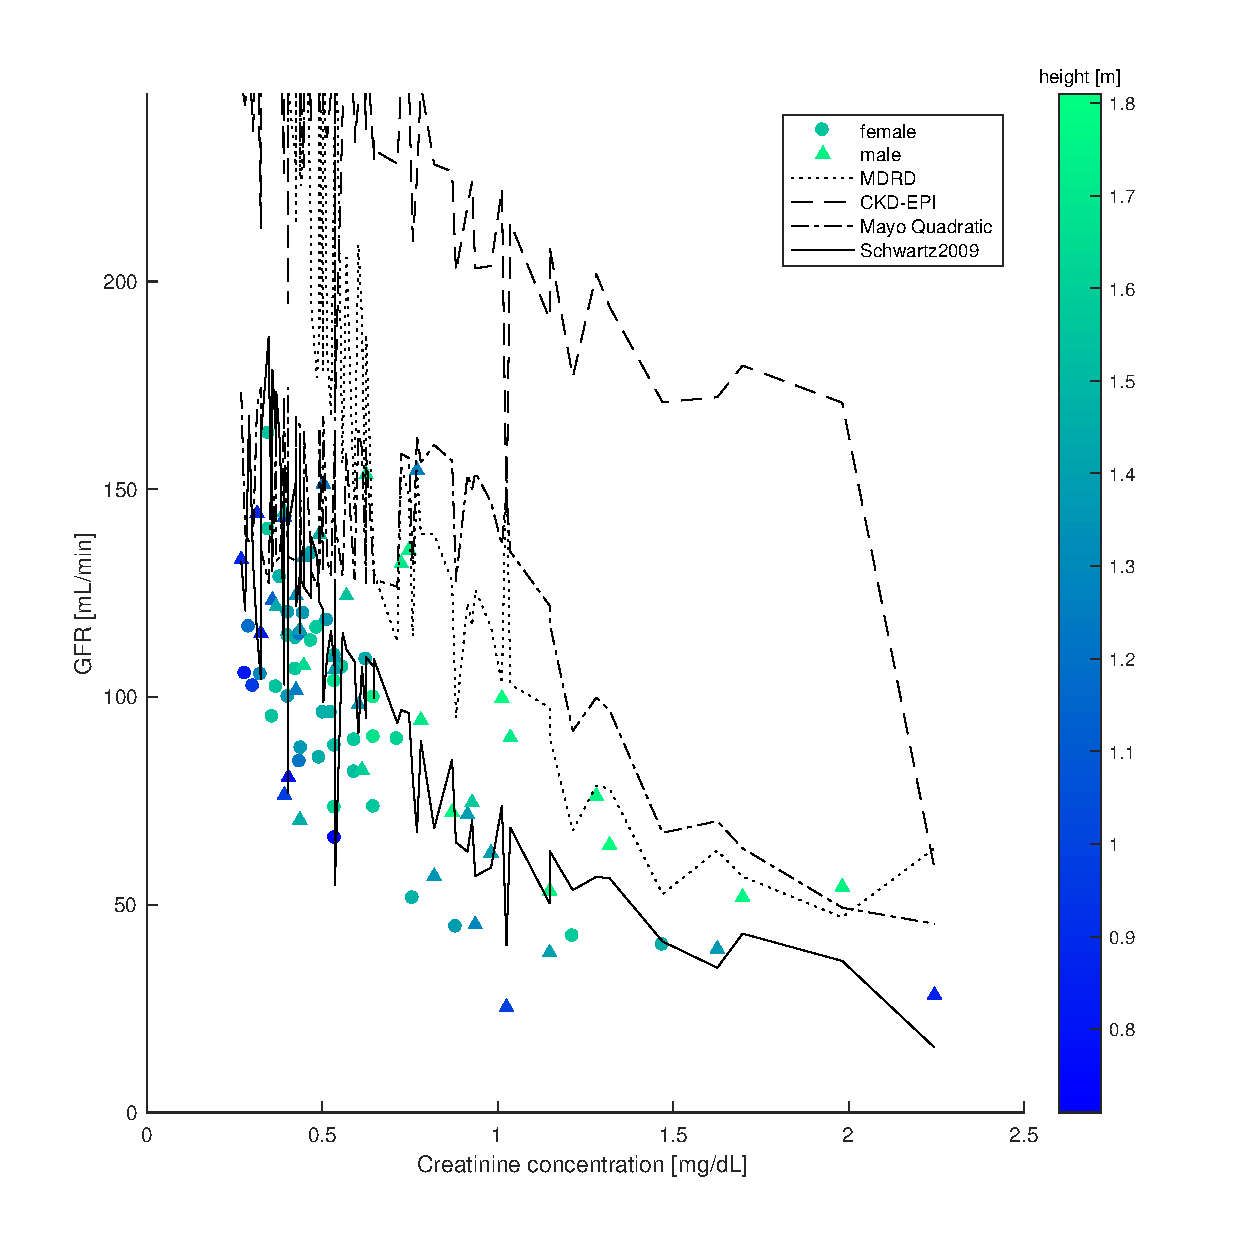
\includegraphics[scale=0.6]{figures/equations}}
  \caption{Comparison of predictions made using different equations (MDRD, CKD-EPI, Mayo Quadratic and updated Schwartz). The serum creatinine concentration refers to the IMDS-traceable values.}
  \label{equations}
\end{figure}

In order to apply SBR, we must first assess the existence of a single dominant variable. This was clearly found to be the serum creatinine concentration. Other variables used to estimate the glomerular filtration rate are age and height, whose effect however is marginal, as the scatter plots in Figure \ref{recessive} reveal no strong statistical features.
%
\begin{figure}[ht]
  \centering
  \makebox[\textwidth][c]{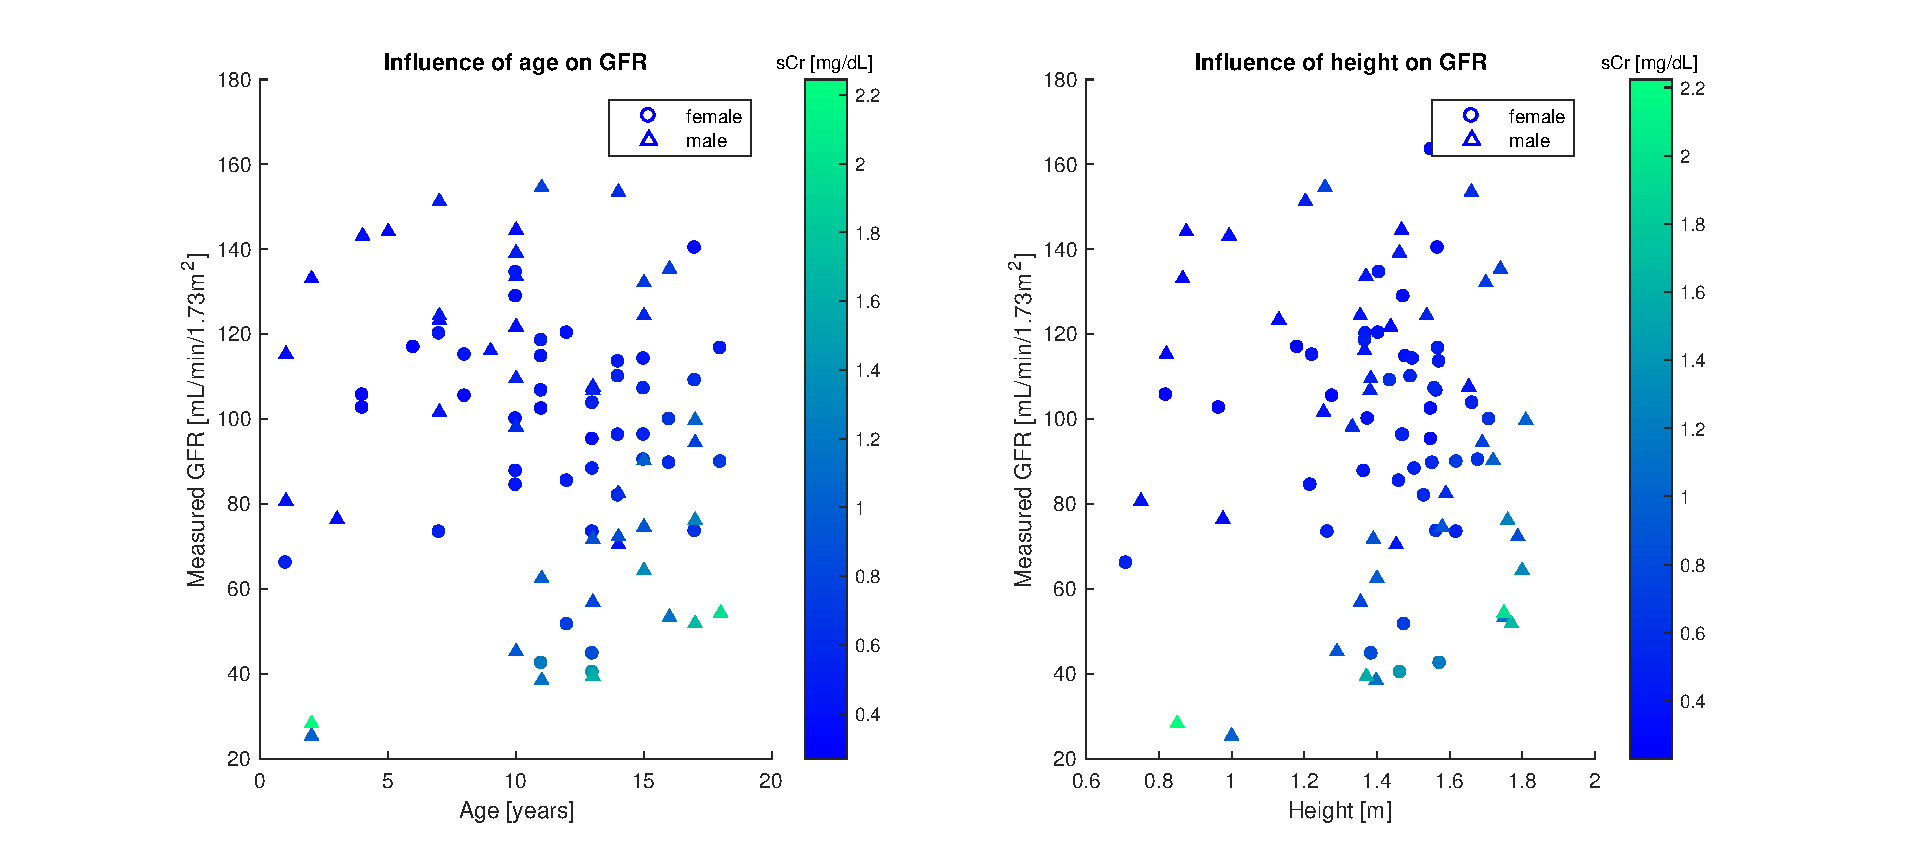
\includegraphics[scale=0.6]{figures/recessive}}
  \caption{Plots of the glomerular filtration rate versus patients age or height suggest weak correlation. The serum creatinine concentration refers to the IMDS-traceable values.}
  \label{recessive}
\end{figure}
%
Quantitatively, this analysis is confirmed by the population correlation coefficient \cite{mukaka}, which, for a generic paired dataset $(z_i, y_i)$ for $i = 1, 2, \ldots, n$ is calculated as
%
\begin{equation}
  \rho_{y,z} = \frac{\sum_{i = 1}^n{(z_i-\bar{z})(y_i-\bar{y})}}
  {\sqrt{\sum_{i=1}^n{(z_i-\bar{z})^2}\sum_{i=1}^n{(y_i-\bar{y})^2}}},
\end{equation}
%
where $\bar{z}=\tfrac{1}{n}\sum_{i=1}^nz_i$ and $\bar{y}=\tfrac{1}{n}\sum_{i=1}^ny_i$. The coefficient of correlation $\rho$ takes values in the interval $[-1,1]$. If variables are directly correlated, then we expect the coefficient to approach $+1$ while, if they are inversely correlated, we expect a value of the coefficient of correlation close to $-1$. Unrelated variables yield a value of $\rho$ close to $0$. Table \ref{corr} shows correlation coefficients between the GFR and each of age, height and sCr for the whole population and the gender-defined subsets.
%
\begin{table}[ht]
  \centering
  \begin{tabular}{|l|c|c|c|}
    \hline
    \textbf{Gender}&$\rho_{\mathit{GFR},sCr}$&$\rho_{\mathit{GFR},age}$&$\rho_{\mathit{GFR},height}$\\
    \hline
    \textrm{Males}     & $-0.7051$ & $-0.1375$ & $-0.0910$  \\
    \hline
    \textrm{Females}   & $-0.7249$ &  $+0.0801$ &  $+0.0548$  \\
    \hline
    \textrm{Both}      & $-0.6744$ & $-0.0565$ & $-0.0425$  \\
    \hline
  \end{tabular}
  \caption{Population correlation coefficients between glomerular filtration rate and age, height and creatinine concentration in patients blood plasma. The serum creatinine concentration refers to the IMDS-traceable values.}
  \label{corr}
\end{table}
%
The results illustrated in the table confirm the weak statistical correlation between glomerular filtration rate and age, as well as between glomerular filtration rate and height, especially for female children.

From the Figure~\ref{equations}, it is readily appreciated that the GFR--sCr relationship presents a monotonically decreasing trend, which enables us to apply the SBR regression algorithm presented in the Section~\ref{blsbr}. According to the observations drawn about the performances of the closed-form models, we did not compare the SBR regression algorithm with the MDRD, the CKD-EPI and the Mayo Quadratic formulas.

As SBR generates a bivariate regression, for the sake of the comparison, a simplified version of the updated Schwartz formula was introduced to be independent of height. This was done by replacing the variable with a constant equal to the mean height of all individuals in the dataset. This model is illustrated in the Figure \ref{regression}, along with the datapoints, the regression curve obtained by SBR using the numerical-algebraic neural system (NANS) method explained in \cite{fiori}, the original updated Schwartz formula and the regression curve obtained using the binning-less method described in Section 2.
%
\begin{figure}[ht]
  \centering
  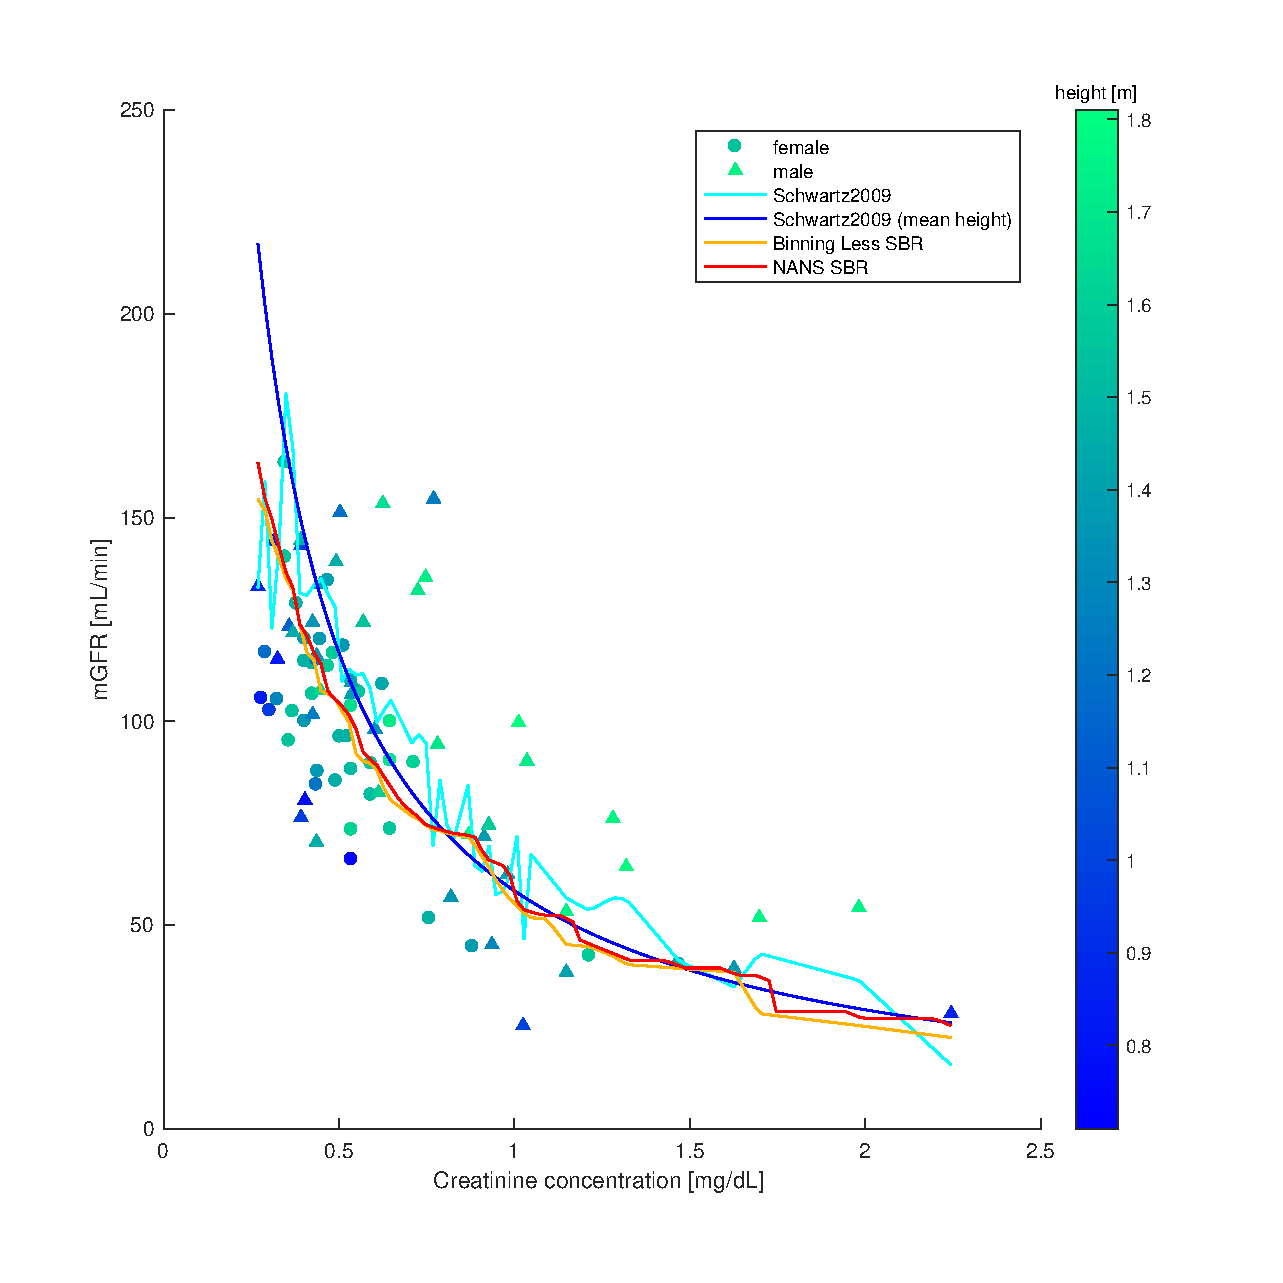
\includegraphics[scale=0.6]{figures/regression}
  \caption{Data set with overlaid regression and estimation curves. Comparison of the updated Schwartz equation, the simplified Schwartz equation, the Numerical-Algebraic Neural System (NANS) method introduced in \cite{fiori} and the proposed method. The serum creatinine concentration refers to the IDMS-traceable values.}
  \label{regression}
\end{figure}

The input-output nature of prediction making systems grants the use of functional notation (e.g. given a value for the independent variable $x$, the prediction made for the value of the dependent variable $y$ can be expressed as $y = f(x)$).
%(e.g. $y = f(x)$, where $x$ is the known independent variable and $y$ is the dependent variable being predicted)
The notation is commonly used in reference to closed-form models and will be adopted in this paper to also indicate predictions made using Algorithm \ref{regression_algo} or by interpolating the curve obtained using the NANS method.

The two closed-form models and the two numerical regression algorithms displayed in the Figure \ref{regression} were compared on prediction performance using three indices: mean squared error (MSE), mean absolute error (MAE) and coefficient of determination ($R^2$).
For a generic prediction making system, represented by the function $f(x)$, being validated over the set of datapoints $\lbrace(x_1,y_1), (x_2,y_2), \ldots, (x_n,y_n)\rbrace$, these indexes are defined as

\begin{eqnarray}
  &&\textit{MSE} = \frac{1}{n}\sum_{i=1}^{n}{(f(x_i)-y_i)^2},\\
  &&\textit{MAE} = \frac{1}{n}\sum_{i=1}^{n}{|f(x_i)-y_i|},\\
  &&R^2 = 1 - \frac{\sum_{i=1}^{n}{(f(x_i)-y_i)^2}}{\sum_{i=1}^{n}{(f(x_i)-\bar{y})^2}},
  \text{ where } \bar{y} = \frac{1}{n}\sum_{i=1}^{n}{y_i}.
\end{eqnarray}

The reference values for a well-performing algorithm are $\textit{MSE}\geq 0$ and $\textit{MAE}\geq 0$ as close as possible to zero and $R^2 \in [0,\ 1]$ as close as possible to $1$ (when $R^2=1$, it is said that a model explains the data perfectly).
In the present context, each $x_i$ represents an instance of serum creatinine concentration sCr, while each $y_i$ represents an instance of glomerular filtration rate GFR, and $n = 87$.
Comparisons were also made to evaluate the generalization ability of the closed-form model (simplified Schwartz) as well as of the considered numerical regression algorithms (SBR and NANS-SBR).
%Comparisons were also made to evaluate the generalization ability of the closed-form models (updated Schwartz and simplified Schwartz) as well as of the considered numerical regression algorithms (SBR and NANS-SBR). 
This was achieved by measuring the ``roughness'' of the the regression curves through the index $G$ defined by
%
\begin{equation}
  G = \sum_{i=3}^{N}{\frac{(f_i-2f_{i-1}+f_{i-2})^2}{N-2}},
\end{equation}
%
on the basis of the second-order differences of a sequence $f_i$. By definition, the index $\textit{G}$ increases with sharp changes in slope. The reference value for a well-performing algorithm is $G\geq 0$ as close as possible to zero. To be useful, the $f_i$ values have to be sorted in some significant manner: in the present context, for each model $f(x)$ to be evaluated, $f_i$ assumes the predictions at $N = 100$ equally spaced, increasing, values of serum creatinine concentration, namely:
%
\begin{equation}\label{eqn_sampl}
  f_i = f\left(x_\mathrm{min} + (i-1)\frac{x_\mathrm{max}-x_\mathrm{min}}{N-1}\right), \text{ for } i = 1,\ \ldots,\ N,
\end{equation}
%
where $x_\mathrm{min}$ and $x_\mathrm{max}$ are respectively the smallest and largest measured creatinine concentration levels. The same index cannot be applied to multivariate functions, therefore the updated Schwartz equation was not tested with this criterion.
%namely
%
%\begin{equation}
%x_\mathrm{min} = \min_{i = 1, \ldots,\ n}\{x_i\},\ x_\mathrm{max} = \max_{i = 1,\ \ldots,\ n}\{x_i\}.
%\end{equation}
%
An index similar to $\mathit{G}$ was discussed in \cite{bishop} to prevent overfitting of a neural-network model.
The value of $G$ is expected to be large for irregular curves and indeed it is close to zero for the simplified Schwartz model (independent of height), which is essentially a hyperbola, graph of a smooth function.
%while it is very high (14.69) for the original Schwartz model, as we are including the effect of a second independent variable (which does contribute to ordering the sequence $f_i$).
%
\begin{table}[ht]
  \centering
  \begin{tabular}{|l|c|c|c|c|}
    \hline
    \textbf{Model}             &$\mathit{G}$  &$\mathit{MSE}$  &$\mathit{MAE}$  &$R^2$    \\
    \hline
    Updated Schwartz           &$ - $ &$863.92$  &$23.19$  &$ 0.1491$  \\
    Simplified Schwartz        &$0.36$  &$1341.80$ &$27.84$  &$-0.3216$  \\
    NANS SBR                   &$1.83$  &$696.62$  &$20.32$  &$ 0.3139$  \\
    Binning-less SBR           &$1.65$  &$674.90$  &$20.19$  &$ 0.3353$  \\
    \hline
  \end{tabular}
  \caption{Generalization/roughness index ($\mathit{G}$), mean squared error ($\mathit{MSE}$), mean absolute error ($\mathit{MAE}$) and coefficient of determination ($R^2$) for the four considered estimation models (updated Schwartz formula, simplified Schwartz formula independent of height, numerical-algebraic neural-system based statistical bivariate regression algorithm, and proposed statistical bivariate regression algorithm). [{\bf\red Nella tabella c'e' qualcosa che non va, perche' $R^2$ non puo' essere negativo.}]}
  \label{regstats}
\end{table}

%The Schwartz2009 model exhibits the lowest $R^2$ value.
The Binning-less statistical bivariate regression algorithm exhibits the lowest $\textit{MSE}$ and $\textit{MAE}$ values, that shows that SBR is very effective at fitting data.
%
\section{Conclusions}\label{conclusion}
%
The aim of the present paper is to discuss the bivariate statistical regression method and to provide an improved algorithm which does not rely on binning for the steps which require estimation of the cumulative distribution functions. The proposed algorithm was compared to the original bivariate statistical regression algorithm based on numerical-algebraic neural systems in the application to a real-world dataset. The considered application is the estimation of an index of kidney function, the glomerular filtration rate, on the basis of regression by the creatinine concentration level in blood plasma. The comparison proved an all-round improvement in the new method, which, aside from being more efficient, yields a closer fit and a smoother regression curve.
%
\begin{thebibliography}{99}
  \bibitem{bestchak} M.J. Best and N. Chakravarti, ``Active set algorithms for isotonic regression; a unifying framework'', \textit{Mathematical Programming}, Vol. 47, pp 425 -- 439, 1990

  \bibitem{bishop} C.M. Bishop, ``Training with noise is equivalent to Tikhonov regularization'', \textit{Neural Computation}, Vol. 7, No. 1, pp. 108 -- 116, 1995

  \bibitem{Counahan} R. Counahan, C. Chantler, S. Ghazali, B. Kirkwood, F. Rose and T.M. Barratt, ``Estimation of glomerular filtration rate from plasma creatinine concentration in children'', \textit{Archives of Disease in Childhood},  Vol. 51, pp. 875 -- 878, 1976

  \bibitem{mgfr2} Z.H. Endre, J.W. Pickering and R.J. Walker, ``Clearance and beyond: the complementary roles of GFR measurement and injury biomarkers in acute kidney injury (AKI)'', \textit{American Journal of Physiology -- Renal Physiology}, Vol. 301, No. 4, pp. F697 -- F707, 2011

  \bibitem{fiori} S. Fiori, ``Fast statistical regression in presence of a dominant independent variable'', \textit{Neural Computing and Applications}, Vol. 22, No. 7, pp. 1367 -- 1378, 2013

  \bibitem{fgl} S. Fiori, T. Gong and H.K. Lee, ``Bivariate nonisotonic statistical regression by a lookup table neural system'', \textit{Cognitive Computation}, Vol. 7, No. 6, pp. 715 -- 730, 2015

  \bibitem{seismic} D. Gao, ``Texture model regression for effective feature discrimination: Application to seismic facies visualization and interpretation'', \textit{Geophysics}, Vol. 69, No. 4, pp. 958 -- 967, 2004

  \bibitem{gfrmed} J. Gill, R. Malyuk, O. Djurdjev and A. Levin, ``Use of GFR equations to adjust drug doses in an elderly multi-ethnic group --- a cautionary tale'', \textit{Nephrology Dialysis Transplantation}, Vol. 22, No. 10, pp. 2894 -- 2899, 2007

  \bibitem{grubb} A. Grubb, S. Blirup-Jensen, V. Lindstrom, C. Schmidt, H. Althau and I. Zegers, ``First certified reference material for cystatin C in human serum ERM-DA471/IFCC'', \textit{Clinical Chemistry and Laboratory Medicine}, Vol. 48, No. 11, pp. 1619 -- 1621, 2010

  \bibitem{book} F.E. Harrell, \textit{Regression modeling strategies: with applications to linear models, logistic and ordinal regression, and survival analysis}, Springer Series in Statistics, 2015

  \bibitem{fat} I. Janssen, P. T Katzmarzyk and R. Ross, ``Waist circumference and not body mass index explains obesity-related health risk', \textit{American Society for Clinical Nutrition}, Vol. 79, pp. 379 -- 384, 2004

  \bibitem{control} R.E. Kopp and R.J. Orford, ``Linear regression applied to system identification for adaptive control systems'', \textit{The American Institute of Aeronautics and Astronautics Journal}, Vol. 1, No. 10, pp. 2300 -- 2306, 1963

  \bibitem{laskin} B.L. Laskin, E. Nehus, J. Goebel, J.C. Khoury, S.M. Davies and S. Jodele, ``Cystatin C-estimated glomerular filtration rate in pediatric autologous hematopoietic stem cell transplantation'', \textit{Biology of Blood and Marrow Transplantation}, Vol. 18, No. 11, pp. 1745 -- 1752, 2012

  \bibitem{MDRD} A.S. Levey, J.P. Bosch, J.B. Lewis, T. Greene, N. Rogers and D. Roth, ``A more accurate method to estimate glomerular filtration rate from serum creatinine: a new prediction equation. Modification of Diet in Renal Disease Study Group'', \textit{Annals of Internal Medicine}, Vol. 130, pp. 461 -- 470, 1999

  \bibitem{ckdepi} A.S Levey, L.A. Stevens, C.H. Schmid, Y.L. Zhang, A.F. Castro III, H.I. Feldman, J.W. Kusek, P. Eggers, F. van Lente, T. Greene and J. Coresh, ``A new equation to estimate glomerular filtration rate'', \textit{Annals of Internal Medicine}, Vol. 150, No. 9, pp. 604 -- 612, 2009

  \bibitem{pava} P. Mair, K. Hornik and J. de Leeuw, ``Isotone Optimization in R: Pool-Adjacent-Violators Algorithm (PAVA) and Active Set Methods``, \textit{Journal of Statistical Software}, Vol. 32, No. 5, pp. 1 -- 24, 2009

  \bibitem{ts} E. Masry, ``Multivariate local polynomial regression for time series: uniform strong consistency and rates'', \textit{Journal of Time Series Analysis}, Vol. 17, pp. 571 -- 599, 1996

  \bibitem{gfralb} K. Matsushita, M. van der Velde, B.C. Astor, M. Woodward, A.S. Levey, P.E. de Jong, J. Coresh and R.T. Gansevoort, ``Association of estimated glomerular filtration rate and albuminuria with all-cause and cardiovascular mortality in general population cohorts: a collaborative meta-analysis'', \textit{The Lancet}, Vol. 375, No. 9731, pp. 2073 -- 2081, 2010

  \bibitem{strontium} J.M. McArthur, R.J. Howarth and T.R. Bailey, ``Strontium isotope stratigraphy: LOWESS version 3: Best fit to the marine Sr-isotope curve for 0-509 Ma and accompanying look-up table for deriving numerical age'', \textit{The Journal of Geology}, Vol. 109, No. 2, pp. 155 -- 170, 2001

  \bibitem{mukaka} M.M. Mukaka, ``A guide to appropriate use of correlation coefficient in medical research'', \textit{Malawi Medical Journal}, Vol. 24, No. 3, pp. 69 -- 71, 2012

  \bibitem{rigalleau} V. Rigalleau, C. Lasseur, C. Raffaitin, C. Perlemoine, N. Barthe, P. Chauveau, C. Combe and H. Gin, ``The Mayo clinic quadratic equation improves the prediction of glomerular filtration rate in diabetic subjects'', \textit{Nephrology Dialysis Transplantation}, Vol. 22, No. 3, pp. 813 -- 818, 2007

  \bibitem{mayo} A.D. Rule, T.S. Larson, E.J. Bergstralh, J.M. Slezak, S.J. Jacobsen and F.G. Cosio, ``Using serum creatinine to estimate glomerular filtration rate: accuracy in good health and in chronic kidney disease'', \textit{Annals of Internal Medicine}, Vol. 141, No. 12, pp. 929 -- 937, 2004

  \bibitem{schwartz} G.J. Schwartz, A. Mu\~{n}oz, M.F. Schneider, R.H. Mak, F. Kaskel, B.A. Warady and S.L. Furth, ``New equations to estimate GFR in Children with CKD'', \textit{Journal of the American Society of Nephrology}, Vol. 20, No. 3, pp. 629 -– 637, 2009

  \bibitem{schwartz3} G.J. Schwartz, M.F. Schneider, P.S. Maier, M. Moxey-Mims, V.R. Dharnidharka, B.A. Warady, S.L. Furth and A. Mu\~{n}oz, ``Improved equations estimating GFR in children with chronic kidney disease using an immunonephelometric determination of cystatin C'', \textit{Kidney International}, Vol. 82, No. 4, pp. 445 -- 453, 2012

  \bibitem{gold} M.A. Serdar, I. Kurt, F. Ozcelik, M. Urhan, S. Ilgan, M. Yenicesu, T. Kutluay, ``A practical approach to glomerular filtration rate measurements: creatinine clearance estimation using cimetidine'', \textit{Annals of Clinical \& Laboratory Science}, Vol. 31, No. 3, pp. 265 -- 273, 2001

  \bibitem{simonsen} O. Simonsen A. Grubb and H. Thysell, ``The blood serum concentration of cystatin C (gamma-trace) as a measure of the glomerular filtration rate'', \textit{Scandinavian Journal of Clinical and Laboratory Investigation}, Vol. 45, No. 2, pp. 97 -- 101, 1985

  \bibitem{jaffe} C. Slot, ``Plasma creatinine determination a new and specific Jaffe reaction method'', \textit{Scandinavian Journal of Clinical and Laboratory Investigation}, Vol. 17, No. 4, pp. 381 -- 387, 1965

  \bibitem{mgfr} I. Soveri, U.B. Berg, J. Bj\"{o}rk, C.G. Elinder, A. Grubb, I. Mejare, G. Sterner and S.E. B\"{a}ck, ``Measuring GFR: A Systematic Review'', \textit{American Journal of Kidney Diseases}, Vol. 64, No. 3, pp. 411 -- 424, 2014

  \bibitem{idms} M.J. Welch, A. Cohen, H.S. Hertz, K.J. Ng, R. Schaffer, P. van der Lijn, and E. White, ``Determination of serum creatinine by isotope dilution mass spectrometry as a candidate definitive method'', \textit{Analytical Chemistry}, Vol. 58, No. 8, pp. 1681 -- 1685, 1986

  \bibitem{gfr} K. Zheng, M. Gong, Y. Qin, H. Song, X. Shi, Y. Wu, F. Li and X. Li, ``Validation of glomerular filtration rate-estimating equations in Chinese children'', \textit{PLoS ONE}, Vol. 12, No. 7, pp. e0180565 (\doi{10.1371/journal.pone.0180565}), 2017
  %
\end{thebibliography}

\begin{appendix}
  \section{MATLAB code to implement the estimating functions}
  \lstinputlisting{../cdf.m}
  \lstinputlisting{../invcdf.m}
  \lstinputlisting{../sbr.m}
\end{appendix}
\end{document}
